In this section we explain the strategy for pulling the fire hose while walking.
%
First, we described the hybrid controller used to control the robot's wrist holding the hose.
%
Then, simulation results are shown for analyzing and demonstrating the robot's behavior when pulling the fire hose while walking.





\subsection{Hybrid controller}			\label{pulling}

\begin{figure}[ht]
 \centering
 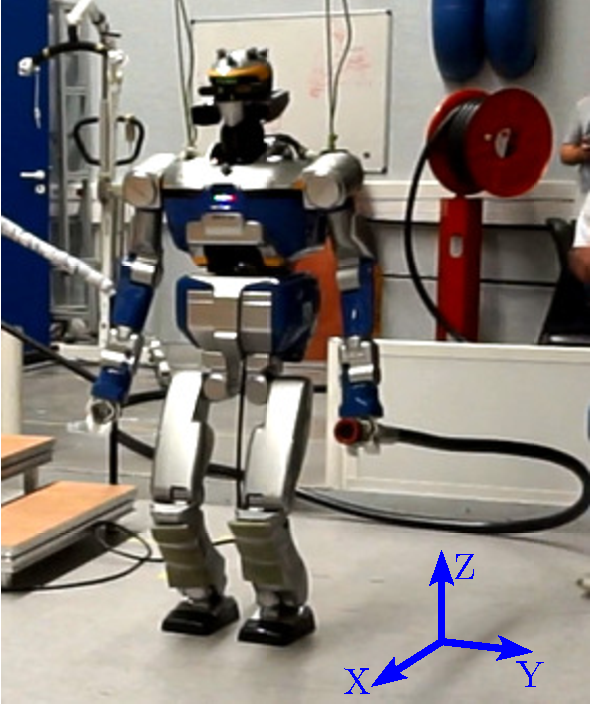
\includegraphics[height=0.40\textwidth]{./figures/coordinates.pdf}
 \vspace{-4mm}
 \caption{The robot coordinate frame.}
 \label{frame}
% \vspace{-5mm}
\end{figure}
%
In order to pull the fire hose while walking a hybrid controller is implemented on the robot's wrist holding the hose.
%
Position control is employed to keep a fix distance between the waist of the robot and it's wrist, and impedance control is employed to pull the hose.
%
According to the frame attached to the robot (as shown in Fig.~\ref{frame}), position control is used in $Y$ direction and impedance control in $X$ and $Z$ directions.
%
%
%
%
% 
%
The impedance controller on the left wrist is defined similarly to the one proposed by Harada et~al. \cite{pushRealTime} as:  
%
\begin{equation}
m\mathbf{\ddot{x}}_{lw} + c\mathbf{\dot{x}}_{lw} = \mathbf{f}_{lw} - \mathbf{f}_d - \mathbf{f}_{\text{pull}} \; ,
\label{eq_imp}
\end{equation}
%
where $\mathbf{x}_{lw} = [x_{lw} \; y_{lw} \; z_{lw}]^T$ represents the robot's left wrist position, and $m$ and $c$ are the desired mass and damping coefficients, respectively.
%
The force applied to the left wrist of the robot is represented by $\mathbf{f}_{lw}$, $\mathbf{f}_d$ is the desired force in the left wrist, and $\mathbf{f}_{\text{pull}}$ represents the desired pulling force, defined as:
%
%
\begin{equation}
\mathbf{f}_{\mathrm{pull}} = \begin{cases}
\mathbf{W} \mathbf{v}^{\mathrm{ref}}	& \quad \mathrm{if} \; z_{la} = z_{ra} = h_a  \\
0  & \quad \mathrm{otherwise} \\
\end{cases}
, 
\label{fpull}
\end{equation}
%
where $z_{la}$ and $z_{ra}$ are the $Z$ direction components of the left and right ankles, $h_a$ is the height of the ankles when making full contact with the floor, $\mathbf{v}^{\text{ref}}$ is the reference velocity vector of the robot when walking and $\mathbf{W}$ is a diagonal matrix.
%
Like this, the robot will pull the hose only at the double support phase when walking and will not pull the hose when standing still.
%
Furthermore, the diagonal matrix $\mathbf{W}$ allows to select in which direction to pull the hose.


The orientation of the wrist will be kept constant with respect to the orientation of the robot's waist, i.e. it will rotate in the same direction, same amount as the robot's waist.


\subsection{Simulation analysis}			\label{sim_pulling}
%
%
\begin{figure}[ht]
 \centering
 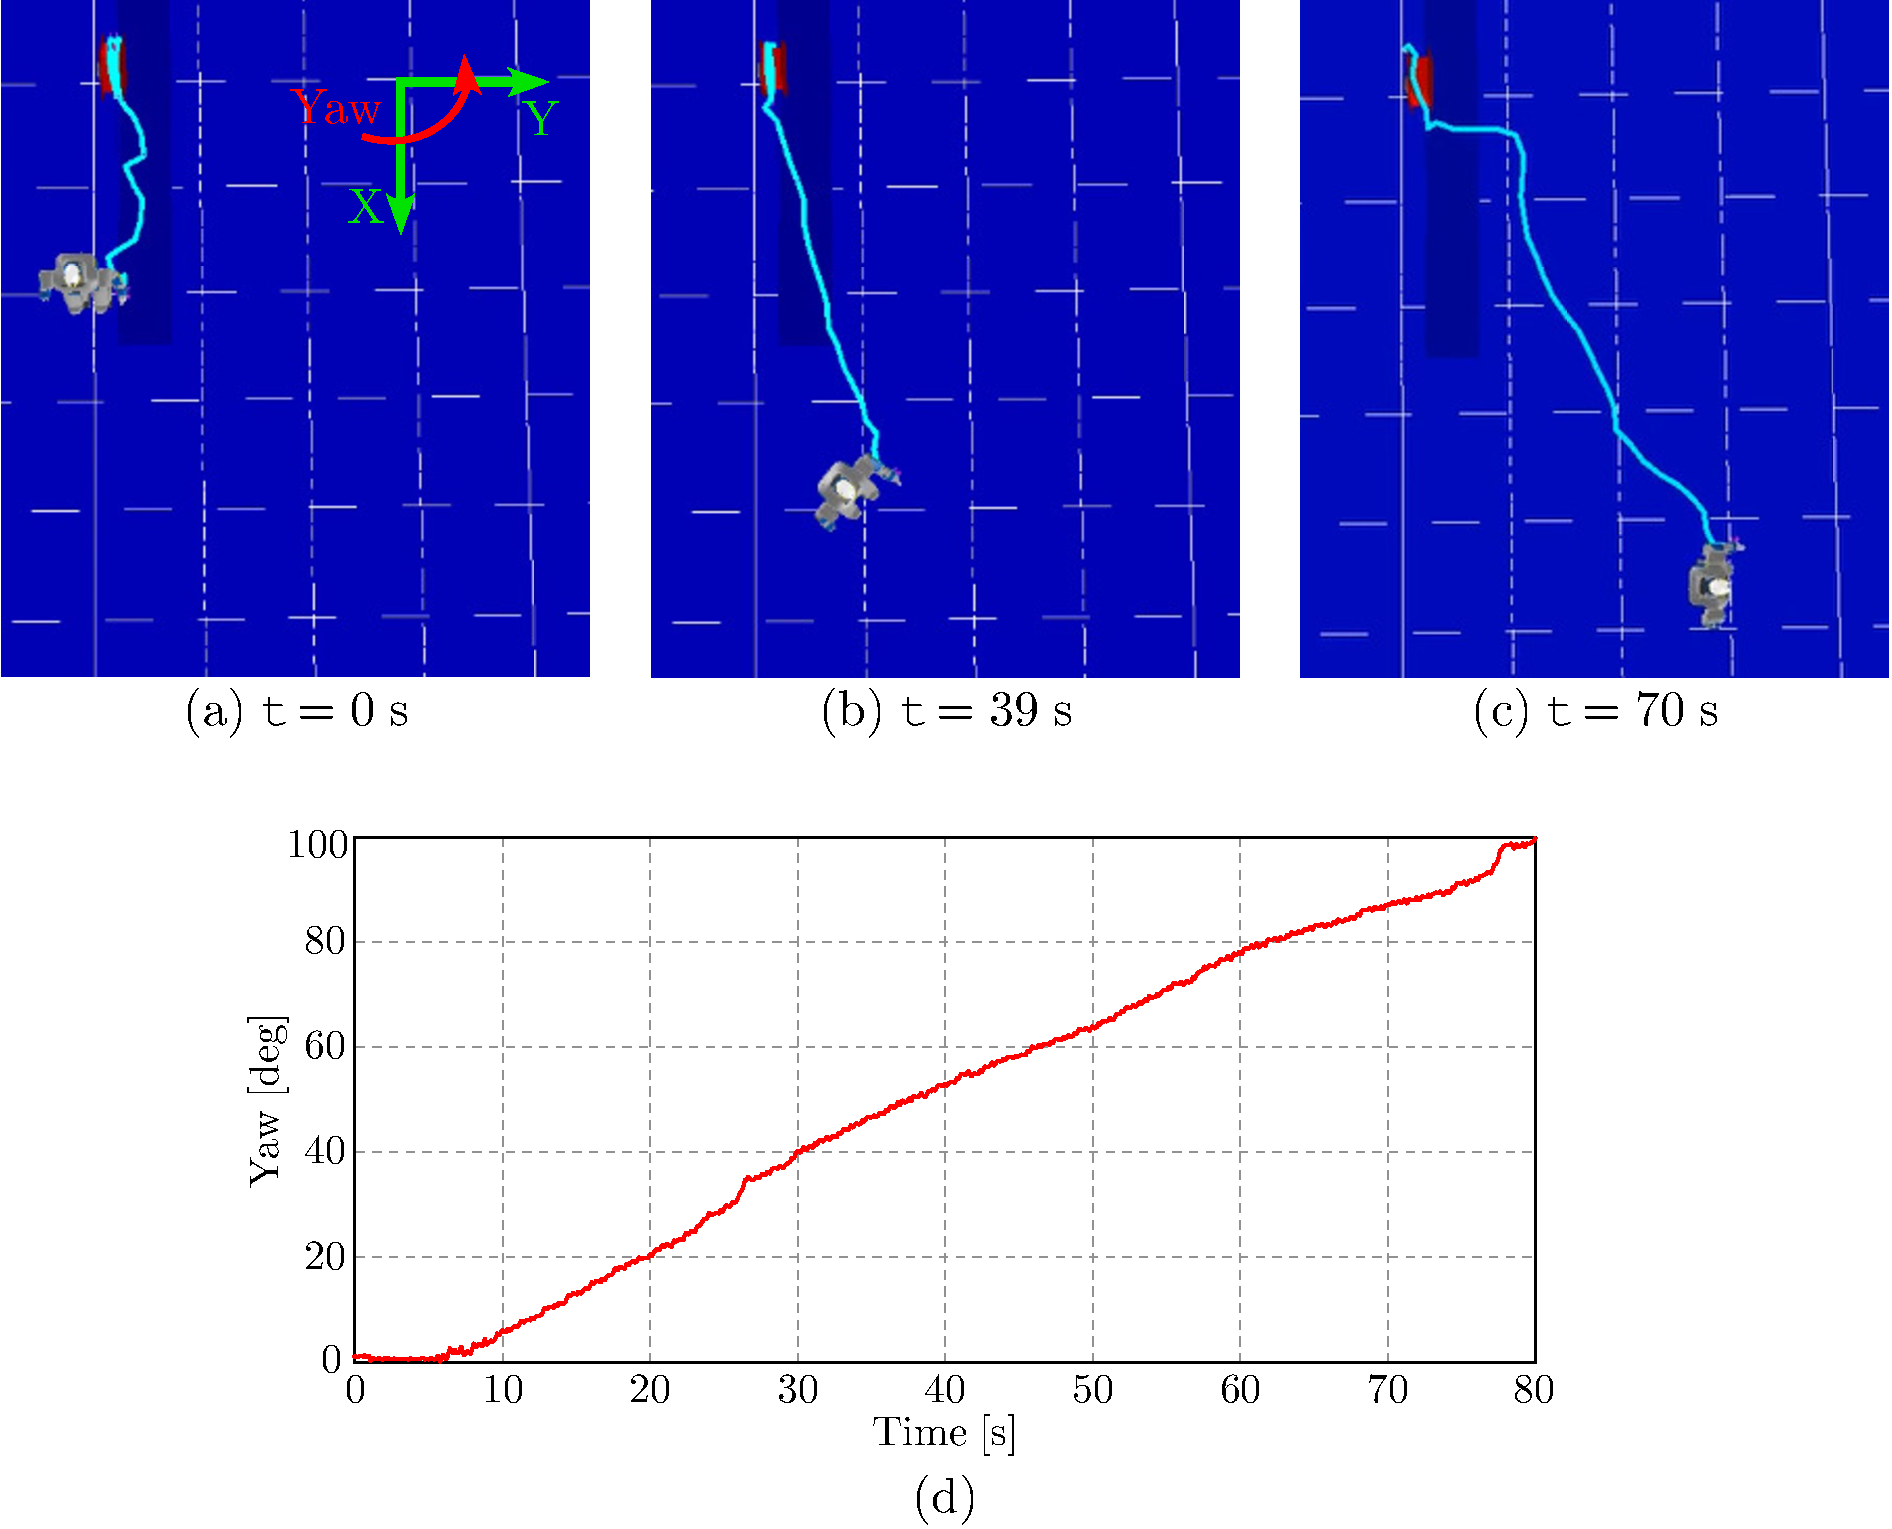
\includegraphics[height=0.40\textwidth]{./figures/yaw_drift_simGraph.pdf}
 \vspace{-3mm}
 \caption{Snapshots of the top view of the simulation of HRP-$2$ robot holding a hose in (a) to (c), and the change in the robot's yaw angle in (d).}
 \label{drift_sim}
% \vspace{-5mm}
\end{figure}
%
%
The humanoid robot HRP-$2$ is simulated using the OpenHRP software version 3.1.2.
This software simulates the dynamics of the hose and HRP-$2$ during the walk.
%
To generate the walking motion of the robot the walking pattern generator described in section \ref{sec_wpg} is used.
%
The fire hose is approximated by a simplified model consisting of rigid cylinders connected by rotational joints with the rotation axis parallel to the cross section of the cylinders.
%

Fig.~\ref{drift_sim} shows the simulation results of the yaw orientation angle of the robot's waist when using a fire hose with a length of $7$ m partially rolled up at the starting time (Fig.~\ref{drift_sim}(a)).
%
The hose has a total mass of $13.2$ kg, which includes the mass of the nozzle and the coupling of the hose.
%
A uniform mass distribution of $1.8$ kg/m, which correspond to the real fire hose, is assumed for the cylinders.
%
The reference velocity given to the pattern generator is $\mathbf v_{\text ref} = [0.1 \; 0.0 \; 0.0]^T$ and it is constant through all the simulation.
%
As it can be seen in Fig.~\ref{drift_sim}, after walking few steps the robot begins to drift to its left with an almost constant velocity.
%
It can be inferred that the force generated by the hose on the robot's wrist generates a slip on the robot's feet, thus generating a drift in the robot's yaw angle.
%


Furthermore, it was discovered that the amount of drift depends on the mass of the fire hose.
%
The change in the yaw angle in simulation using hoses with different weights is shown in Fig.~\ref{drift_sim2}.
%
The light, normal an heavy hoses have a total mass of $4.52$, $9.04$ and $13.56$ kg, respectively and a length of $1.8$ m for each of them.
%
From this results it can be observed that the drift on the orientation of the robot depends on the disturbance given by pulling the hose on its left wrist.
%
%
\begin{figure}[t]
 \centering
 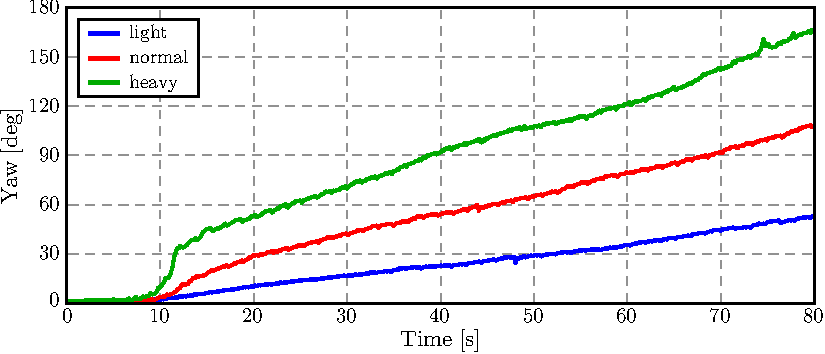
\includegraphics[height=0.3\textwidth]{./figures/yaw_drifts_3weights.pdf}
 \vspace{-3mm}
 \caption{Change in the robot's yaw angle for three different weights per length unit. Light's hose mass is $4.52$ kg, normal's hose mass is $9.04$ kg and heavy's mass is $13.56$ kg}
 \label{drift_sim2}
% \vspace{-5mm}
\end{figure}


